\section{Temporal Action Proposals}
\par The task of Temporal Action Proposals involves generating temporal segments in long untrimmed video. Given a video, the model should be able to output temporal intervals (timestamps) that have a possibility of containing an action. Buch \textit{et al} \cite{buch2017sst} used Single-Stream Temporal Action Proposal (SST) that does not require division of input video into a number of short clips or use of overlapping sliding windows. The method uses a GRU-based sequence encoder which processes the video in a single pass and at each time step outputs proposals and their confidences by utilizing the C3D encoded features of the video frames. The model however had an issue of predicting an output segment which contains several ground-truth segments. Lin \textit{et al} \cite{lin2019bmn} develop a Boundary-Matching Mechanism for efficiently evaluating the proposals from a bottom-up generators and give reliable confidence scores.

\section{Transformers in Computer Vision}
\par Transformers \cite{tfm} have been widely used in applications requiring processing of sequential data like language or speech. Various solutions have been coming forward to utilize this generalized architectures in the domain of computer vision. Dosovitskiy \textit{et al} \cite{dosovitskiy2020vit} used only transformers (called Vision Transformers or ViT), without any CNN backbone for the task of image classification. The model divided an image into fixed-size patches and pass them along with an extra learnable class embedding token as input to a tranformer encoder. The output of the class embedding token is then feed to a MLP head to get the output object class. The approach suffers from the issues of less scalability and larger running time, since the number of tokens is highly dependent on the input resolution of the image. Liu \textit{et al} \cite{liu2021swin} tackles these issues by intoducing a hierarchical transformer called Swin-Transformer. The method uses shifted windows to limit the attention computation to non-overlapping local windows. It decreases the quadratic complexity of ViT to linear comutational complexity with respect to the input image size. Fayyaz \textit{et al} \cite{fayyaz2021ats} introduces a parameter free Adaptive Token Sampling (ATS) module which can be plugged into any ViT models and reduce the GFLOPs without any additional training. The proposed method decides and selects the right amount of tokens to attend to. 
\par Carion \textit{et al} \cite{carion2020detr} develop DEtection TRansformer (DETR) for the task of object detection or panoptic segmentation in images. The method completely eradicates the need of developing various hand-designed features like anchors, non-max supression thresholds, etc. It is an end-to-end architecture viewing object detection task as set prediction task. The model tokenizes the input image using a CNN backbone (ResNet-50) and passes it to the transformer encoder along with positional embeddings. The output of encoder is given to the decoder along with learnable positional embeddings refered to as object queries. The decoder outputs the query features which are passed to a shared Feed Forward Network (FFN) that predicts the object bounding box and class. They use Hungarian Bipartite Matcher to compute the loss between ground truth and prediction. DETR inspite of comparable performance with other state-of-the-art CNN architectures, faced issues of slower convergence because of global attention in encoder and inaccuracy in detection of smaller objects. A number of approaches were introduced for handling this issue. Zhu \textit{et al} \cite{zhu2020deformable} proposed Deformable DETR which answers both the issues by using Multi-scale Feature Maps of the input image and attending to limited number of tokens in encoder. The method also introduced variations for better accuracy, namely iterative bounding box refinement and two-stage Deformable DETR. The model required 10x faster convergence and is 1.6x faster than the original DETR. This however does increase the input tokens by 20x because of multi-scale features. Roh \textit{et al} \cite{roh2021sparse} make Deformable DETR further efficient by selectively updating only the tokens that are expected to be referenced by the DETR decoder. This is done by learning a scoring network for predicting binarized Decoder cross-Attention Map (DAM). The model also improves the gradient flow throughout the transformer by introducing encoder-auxiliary loss. Sparse-DETR along with Swin Transformer Backbone increases the FPS by 38\% as compared to Deformable DETR.


\section{Dense Video Captioning}
\par The problem of dense video captioning was introduced by Krishna \textit{et al} in \cite{krishna2017densecaptioning} by proposing ActivityNet Captions dataset. Their architecture involved a proposal module and captioning module. The proposal module was inspired from DAPs \cite{Escorcia2016DAPsDA}, while the captioning module incorporated LSTM with contextual features along with event feature as inputs. The architecture was able to detect events and generate captions of the video in a single pass without the need of a time consuming sliding window approach.  However, since the features were dependent on the end location of the event, the model generated same captions for events ending at same timestamp.

\begin{figure}[h]
	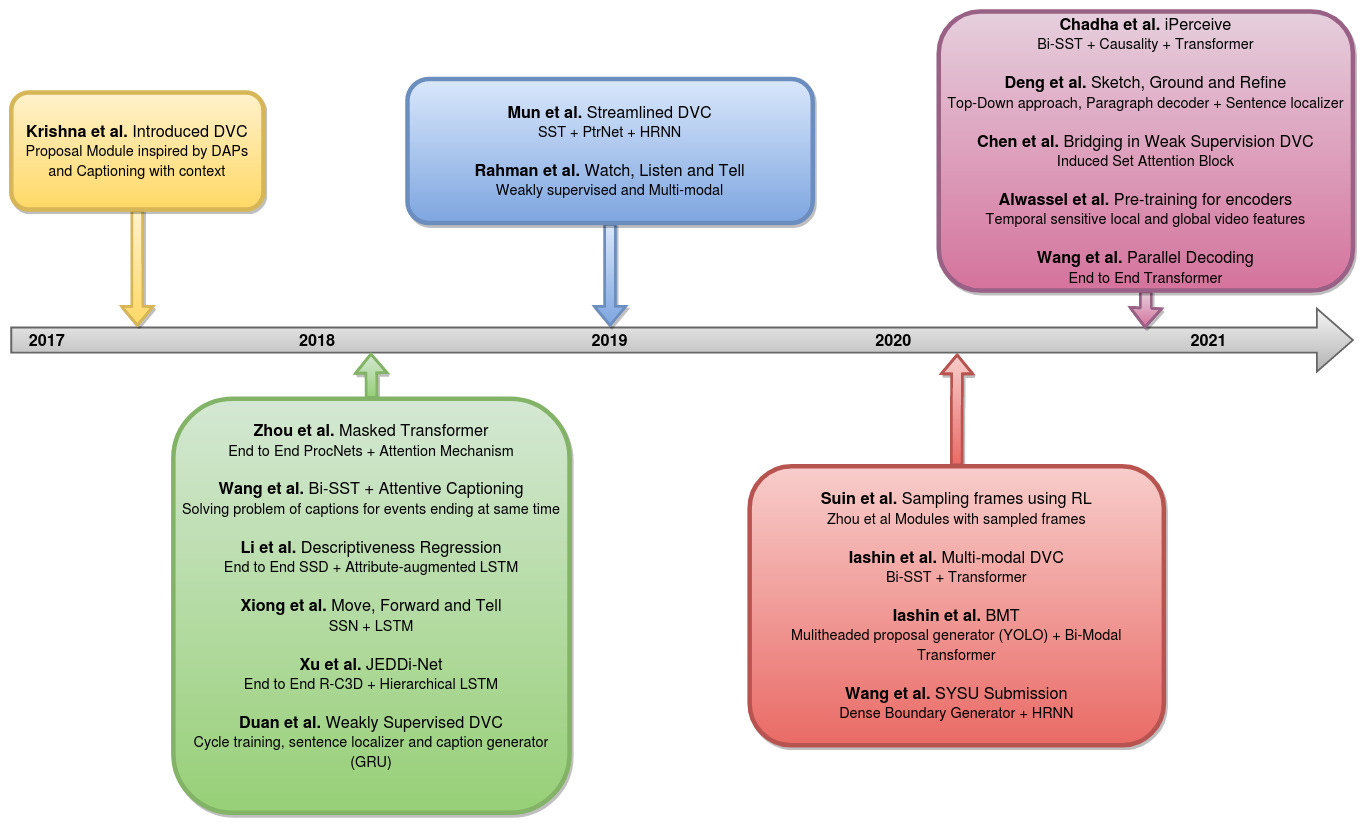
\includegraphics[width=\linewidth]{assets/img/timeline.jpg}
	\caption{Evolution of dense video captioning methods over time.}
\end{figure}

\par Following the release of ActivityNet Captions dataset in 2017, many researchers were able to surpass the results of baseline model and achieve state-of-the-art. Zhou \textit{et al} \cite{zhou2018end} addressed the problem of little influence of language desciptions on event proposals if the two modules are trained separately. They introduced an end-to-end masked transformer for propogating captioning error to proposal module for better performance. Furthermore, they proposed a self-attention mechanism for learning long-range dependencies in video. The proposal module was based on ProcNets \cite{zhou2017automatic}. The caption decoder employed a differentiable proposal mask to account for features in the respective event. Wang \textit{et al} \cite{wang2018bidirectional} employed Bi-SST as their proposal generator to account for past and future context information. The captioning module consisted of attentive fusion of context features, the weights of which were decided by a context gating mechanism. The architecture selected final captions based on joint ranking method which accounted for both proposal and caption confidence. Li \textit{et al} \cite{li2018jointly}, inspired by object localization networks like \cite{ren2016faster, liu2016ssd}, presented an end-to-end model with descriptiveness regression. An attribute-augmented LSTM network optimized using reinforcement learning was used for captioning module. Xiong \textit{et al} \cite{xiong2018forward} strived to generate relevant, coherent and concise descriptions using SSN \cite{zhao2017temporal} for event localization and LSTM for event selection and caption generation. Reinforcement learning with sentence-level reward is used to train the captioning network. Xu \textit{et al} \cite{xu2018joint} proposed JEDDi-Net, an end-to-end architecture incorporating visual and language contexts. Segment Proposal Network inspired from R-C3D \cite{xu2017rc3d} is used for proposal generation. Hierarchical LSTM with caption-level controller network and word-level sentence decoder is used for caption generation. The proposal features are represented using 3D Segment-of-Interest Pooling. Duan \textit{et al} \cite{duan2018weakly} introduced weak supervision training with no need of temporal annotations of events. They trained sentence localizer and caption generator in cyclic manner minimizing the reconstruction loss. However, the method struggles to detect beginning of events properly.

\par Mun \textit{et al} \cite{mun2019streamlined} tackles the challenge of coherent captioning by considering temporal dependency between events. They used SST for event proposals, PtrNet for event sequence generation and HRNN for captioning. Rahman \textit{et al} \cite{rahman2019watch} utilized weak supervision method from \cite{duan2018weakly} and were the first to try multi-modal approach for dense video captioning. They show how audio alone can be competitive to the previous visual based results. The paper also discusses various methods to encode audio (MFCC, CQT, SoundNet) and context fusion techniques for multiple modalities (Multiplicative Mixture, Multi-modal context fusion, MUTAN). The architecture suffered from proposal localization accuracy due to weak supervision. Furthermore, the results are also affected due to unavailability of part of the dataset as some videos are not available on their respective urls.

\par \sloppy Suin \textit{et al} \cite{suin2020efficient} aimed to reduce computational cost by processing fewer frames. They used deep reinforcement-based approach to describe multiple events in a video by watching a portion of the frames. The event proposal and captioning modules were inspired from \cite{zhou2018end}. Iashin \textit{et al} \cite{iashin2020multimodal} shows the importance of audio and speech modalities alongside visual features for dense video captioning task. They employ a Bi-SST for proposal and the captioning module consists of a Transformer architecture with three blocks: an encoder, decoder and generator. The model was able to achieve better performance than the then existing methods despite of unavailability of full dataset for multiple modalities. Iashin \textit{et al} \cite{iashin2020better} utilized audio and video with Bi-modal Transformer for captioning. The proposal generator consisted of multiheaded method, inspired from YOLO object detector \cite{yolo}. Their ablation analysis depicted stronger contribution of visual cues alone than audio cues alone. However, both modalities combined gave better results. Wang \textit{et al} \cite{wang2020densecaptioning} adapt DBG \cite{lin2019fast} for temporal event proposals alongwith ESGN \cite{mun2019streamlined} for candidate subset selection. The captioning module consists of an encoder-decoder architecture with CMG (cross-modal gating) block to adaptively balance the visual and linguistic information.

\par Chadha \textit{et al} \cite{chadha2020iperceive} proposed to handle cognitive error (causality between events) and incorrect attention (attending to objects in the frame). Their end-to-end model consisted of Bi-SST for proposals, Common-Sense Reasoning for causality learning and Transformer based architecture \cite{iashin2020multimodal} for captioning. The common-sense reasonining module employed a borrow-put experiment for determining dependency between events and generate context-aware features. Deng \textit{et al} \cite{deng2021sketch} introduced a top-down approach, reversing the usual detect-then-describe method. The architecture first generates a multi-sentence paragraph to describe the whole video and then localize each sentence for events. The captions are then refined using dual-path cross attention module. The top-down approach increased coherency in captions. Chen \textit{et al} \cite{chen2021towards} worked on closely bridging event localization and captioning modules for weakly supervised learning. The Induced Set Attention Block helps the captioner to learn highly abstracted global structure of the video. The method suffers from detecting visually small concepts/objects. Alwassel \textit{et al} \cite{alwassel2021tsp} introduce a supervised pre-training  paradigm for temporal action localization. The paradigm also considers background clips and global video information, to improve temporal sensitivity. Wang \textit{et al} \cite{wang2021endtoend} formulated dense video captioning as a set prediction task and introduced an end-to-end dense video captioning framework with parallel decoding (PDVC). PDVC adopts the vision transformer to learn attentive interaction of different frames. Two prediction heads run in parallel over query features, leveraging the mutual benefits between two tasks of localization and captioning.

% Please add the following required packages to your document preamble:
% \usepackage{multirow}
\begin{table}[]
	\begin{tabular}{|c|c|cccc|cccc|}
		\hline
		\multirow{2}{*}{\textbf{Paper}}          & \multirow{2}{*}{\textbf{Set}} & \multicolumn{4}{c|}{\textbf{Ground Truth Proposals}}                                                                          & \multicolumn{4}{c|}{\textbf{Learnt Proposals}}                                                                       \\ \cline{3-10} 
		&                               & \multicolumn{1}{c|}{\textbf{M}} & \multicolumn{1}{c|}{\textbf{C}} & \multicolumn{1}{c|}{\textbf{B@3}} & \textbf{B@4}          & \multicolumn{1}{c|}{\textbf{M}} & \multicolumn{1}{c|}{\textbf{C}} & \multicolumn{1}{c|}{\textbf{B@3}} & \textbf{B@4} \\ \hline
		\multirow{2}{*}{Krishna \textit{et al} \cite{krishna2017densecaptioning} DCE}             & Validation                    & \multicolumn{1}{c|}{8.88}       & \multicolumn{1}{c|}{25.12}      & \multicolumn{1}{c|}{4.09}         & 1.60                  & \multicolumn{1}{c|}{5.69}       & \multicolumn{1}{c|}{12.43}      & \multicolumn{1}{c|}{1.90}         & 0.71         \\ \cline{2-10} 
		& Test                          & \multicolumn{1}{c|}{9.46}       & \multicolumn{1}{c|}{24.56}      & \multicolumn{1}{c|}{7.12}         & 3.98                  & \multicolumn{1}{c|}{4.82}       & \multicolumn{1}{c|}{17.29}      & \multicolumn{1}{c|}{3.86}         & 2.20         \\ \hline
		\multirow{2}{*}{Zhou \textit{et al} \cite{zhou2018end} Masked Transformer} & Validation                    & \multicolumn{1}{c|}{11.16}      & \multicolumn{1}{c|}{47.71}      & \multicolumn{1}{c|}{5.76}         & 2.71                  & \multicolumn{1}{c|}{4.98}       & \multicolumn{1}{c|}{9.25}       & \multicolumn{1}{c|}{2.42}         & 1.15         \\ \cline{2-10} 
		& Test                          & \multicolumn{1}{c|}{10.12}      & \multicolumn{1}{c|}{}           & \multicolumn{1}{l|}{}             & \multicolumn{1}{l|}{} & \multicolumn{1}{c|}{10.12}      & \multicolumn{1}{l|}{}           & \multicolumn{1}{c|}{}             &              \\ \hline
		\multirow{2}{*}{Wang \textit{et al} \cite{wang2018bidirectional} Bi-SST}             & Validation                    & \multicolumn{1}{c|}{10.89}      & \multicolumn{1}{c|}{}           & \multicolumn{1}{c|}{}             &                       & \multicolumn{1}{c|}{5.86}       & \multicolumn{1}{c|}{7.99}       & \multicolumn{1}{c|}{2.55}         & 1.31         \\ \cline{2-10} 
		& Test                          & \multicolumn{1}{c|}{}           & \multicolumn{1}{c|}{}           & \multicolumn{1}{l|}{}             & \multicolumn{1}{l|}{} & \multicolumn{1}{c|}{9.65}       & \multicolumn{1}{l|}{}           & \multicolumn{1}{c|}{}             &              \\ \hline
		\multirow{2}{*}{Li \textit{et al} \cite{li2018jointly} Descriptivness Regr.} & Validation                    & \multicolumn{1}{c|}{10.33}      & \multicolumn{1}{c|}{26.26}      & \multicolumn{1}{c|}{4.55}         & 1.71                  & \multicolumn{1}{c|}{6.93}       & \multicolumn{1}{c|}{13.21}      & \multicolumn{1}{c|}{2.27}         & 0.74         \\ \cline{2-10} 
		& Test                          & \multicolumn{1}{c|}{}           & \multicolumn{1}{c|}{}           & \multicolumn{1}{l|}{}             & \multicolumn{1}{l|}{} & \multicolumn{1}{c|}{12.96}      & \multicolumn{1}{l|}{}           & \multicolumn{1}{c|}{}             &              \\ \hline
		Xu \textit{et al} \cite{xu2018joint} JEDDi-Net                             & Test                          & \multicolumn{1}{c|}{}           & \multicolumn{1}{c|}{}           & \multicolumn{1}{c|}{4.06}         & 1.63                  & \multicolumn{1}{c|}{8.58}       & \multicolumn{1}{c|}{19.88}      & \multicolumn{1}{c|}{4.06}         & 1.63         \\ \hline
		\multirow{2}{*}{Mun \textit{et al} \cite{mun2019streamlined} Streamlined DVC}     & Validation                    & \multicolumn{1}{c|}{13.07}      & \multicolumn{1}{c|}{43.48}      & \multicolumn{1}{c|}{4.41}         & 1.28                  & \multicolumn{1}{c|}{8.82}       & \multicolumn{1}{c|}{30.68}      & \multicolumn{1}{c|}{2.94}         & 0.93         \\ \cline{2-10} 
		& Test                          & \multicolumn{1}{c|}{}           & \multicolumn{1}{c|}{}           & \multicolumn{1}{l|}{}             & \multicolumn{1}{l|}{} & \multicolumn{1}{c|}{8.19}       & \multicolumn{1}{l|}{}           & \multicolumn{1}{c|}{}             &              \\ \hline
		Duan \textit{et al} \cite{duan2018weakly} Weakly Supervised DCE               & Test                          & \multicolumn{1}{c|}{}           & \multicolumn{1}{c|}{}           & \multicolumn{1}{c|}{2.62}         & 1.27                  & \multicolumn{1}{c|}{6.3}        & \multicolumn{1}{c|}{18.77}      & \multicolumn{1}{c|}{2.62}         & 1.27         \\ \hline
		Rahman \textit{et al} \cite{rahman2019watch} Watch, Listen, Tell               & Validation *                  & \multicolumn{1}{c|}{7.23}       & \multicolumn{1}{c|}{25.36}      & \multicolumn{1}{c|}{3.04}         & 1.46                  & \multicolumn{1}{c|}{4.93}       & \multicolumn{1}{c|}{13.79}      & \multicolumn{1}{c|}{1.85}         & 0.9          \\ \hline
		Suin \textit{et al} \cite{suin2020efficient} Efficient framework for DVC         & Validation                    & \multicolumn{1}{c|}{}           & \multicolumn{1}{c|}{}           & \multicolumn{1}{c|}{2.87}         & 1.35                  & \multicolumn{1}{c|}{6.21}       & \multicolumn{1}{c|}{13.82}      & \multicolumn{1}{c|}{2.87}         & 1.35         \\ \hline
		Iashin \textit{et al} \cite{iashin2020multimodal} Multi-modal DVC                   & Validation *                  & \multicolumn{1}{c|}{11.72}      & \multicolumn{1}{c|}{}           & \multicolumn{1}{c|}{5.83}         & 2.86                  & \multicolumn{1}{c|}{7.31}       & \multicolumn{1}{l|}{}           & \multicolumn{1}{c|}{2.6}          & 1.07         \\ \hline
		Iashin \textit{et al} \cite{iashin2020better} BMT                               & Validation *                  & \multicolumn{1}{c|}{10.90}      & \multicolumn{1}{c|}{}           & \multicolumn{1}{c|}{4.63}         & 1.99                  & \multicolumn{1}{c|}{8.44}       & \multicolumn{1}{l|}{}           & \multicolumn{1}{c|}{3.84}         & 1.88         \\ \hline
		Xiong \textit{et al} \cite{xiong2018forward} Move Forward and Tell              & Validation                    & \multicolumn{1}{c|}{}           & \multicolumn{1}{c|}{}           & \multicolumn{1}{c|}{2.84}         & 1.24                  & \multicolumn{1}{c|}{7.08}       & \multicolumn{1}{l|}{}           & \multicolumn{1}{c|}{2.84}         & 1.24         \\ \hline
		\multirow{2}{*}{Wang \textit{et al} \cite{wang2020densecaptioning} SYSU}               & Validation                    & \multicolumn{1}{c|}{14.85}      & \multicolumn{1}{c|}{}           & \multicolumn{1}{l|}{}             & \multicolumn{1}{l|}{} & \multicolumn{1}{c|}{10.31}      & \multicolumn{1}{l|}{}           & \multicolumn{1}{c|}{}             &              \\ \cline{2-10} 
		& Test                          & \multicolumn{1}{c|}{}           & \multicolumn{1}{c|}{}           & \multicolumn{1}{l|}{}             & \multicolumn{1}{l|}{} & \multicolumn{1}{c|}{9.28}       & \multicolumn{1}{l|}{}           & \multicolumn{1}{c|}{}             &              \\ \hline
		Chadha \textit{et al} \cite{chadha2020iperceive} iPerceive                         & Validation *                  & \multicolumn{1}{c|}{12.27}      & \multicolumn{1}{c|}{}           & \multicolumn{1}{c|}{6.13}         & 2.98                  & \multicolumn{1}{c|}{7.87}       & \multicolumn{1}{l|}{}           & \multicolumn{1}{c|}{2.93}         & 1.29         \\ \hline
		Deng \textit{et al} \cite{deng2021sketch} Sketch, Ground and Refine           & Validation                    & \multicolumn{1}{c|}{}           & \multicolumn{1}{c|}{}           & \multicolumn{1}{l|}{}             & 1.67                  & \multicolumn{1}{c|}{9.37}       & \multicolumn{1}{c|}{22.12}      & \multicolumn{1}{c|}{}             & 1.67         \\ \hline
		Chen \textit{et al} \cite{chen2021towards} Towards Bridging EC-SL              & Validation                    & \multicolumn{1}{c|}{}           & \multicolumn{1}{c|}{}           & \multicolumn{1}{c|}{2.78}         & 1.33                  & \multicolumn{1}{c|}{7.49}       & \multicolumn{1}{c|}{21.21}      & \multicolumn{1}{c|}{2.78}         & 1.33         \\ \hline
		\textbf{Alwassel \textit{et al} \cite{alwassel2021tsp} TSP with BMT}           & Validation                    & \multicolumn{1}{c|}{}           & \multicolumn{1}{c|}{}           & \multicolumn{1}{c|}{4.16}         & 2.02                  & \multicolumn{1}{c|}{8.75}       & \multicolumn{1}{l|}{}           & \multicolumn{1}{c|}{4.16}         & 2.02         \\ \hline
		Wang \textit{et al} \cite{wang2021endtoend} Parallel decoding                   & Validation *                  & \multicolumn{1}{c|}{11.26}      & \multicolumn{1}{c|}{53.65}      & \multicolumn{1}{l|}{}             & 3.12                  & \multicolumn{1}{c|}{8.08}       & \multicolumn{1}{c|}{28.59}      & \multicolumn{1}{c|}{}             & 1.96         \\ \hline
	\end{tabular}

\centering
\caption{Performance comparison of previous methods on the ActivityNet Captions dataset (* some videos unavailable)}  \label{tab: performance-comparison}

\end{table}

\section{Identified Themes}
\par Dense video captioning can be decomposed into two parts: event localization and event description. Existing research methodologies can be grouped into different categories based on training methods, modalities used and ordering of tasks.

\subsection{Based on Training schemes}
\begin{enumerate}
	\item \textbf{Independent training}: Training the proposal and captioning module independently, with no loss propogation or interaction between the two.
	\item \textbf{Alternate training}: alternate between i) training the proposal module only and ii) training the captioning module on the positive event proposals while fine-tuning the proposal module.
	\item \textbf{End-to-End}: Training the proposal and captioning module together, with caption information being able to affect and improve localization capability in the video.
	\item \textbf{Weakly Supervised}: Training the model without ground-truth annotations of temporal events. This method assumes one-to-one correspondence between i.e. each caption describes one temporal event, and each temporal event has one caption.
\end{enumerate}

\subsection{Based on Modalities}
\begin{enumerate}
	\item \textbf{Uni-modal}: Utilizes only one type of input feature. For example, only visual features.
	\item \textbf{Multi-modal}: Utilizes more than one type of input features. For example, combinations of visual, audio and speech features.
\end{enumerate}

\subsection{Based on Task ordering}
\begin{enumerate}
	\item \textbf{Top-Down}: \textit{localize-then-describe}. Predicts the temporal intervals and then caption them. May include optional postprocessing such as ranking proposals, extracting top-k proposals based on confidence scores, etc.
	\item \textbf{Bottom-Up}: \textit{describe-localize-refine}. Describes the entire video into a paragraph using Video Paragraph Generation models. Then localize each sentence from the paragraph over the video. The localized boundaries are then used to re-caption the event.
\end{enumerate}

\section{Datasets}
\addtocontents{toc}{\protect\setcounter{tocdepth}{1}}
\subsection{Textually Annotated Cooking Scenes (TACoS)}

\par TACoS is a subset of MP-II Composites. It was then processed further to provide coherent textual descriptions for high-quality videos. The TACoS dataset was created by filtering through MP-II Composites and limiting the activities to those that involve the manipulation of cooking ingredients and have at least four videos for the same activity. As a result, TACoS includes 26 fine-grained cooking activities spread across 127 videos. Twenty different textual descriptions were collected for each video. The dataset consists of 11,796 sentences with 17,334 action descriptions. The dataset also allows for the alignment of sentences describing activities by obtaining approximate time stamps for the beginning and end of each activity.

\subsection{TACoS-MultiLevel}

\par The TACoS corpus was used to collect TACoS-MultiLevel. Three levels of descriptions were collected for each video in the TACoS corpus: (1) a detailed description of the video with no more than 15 sentences per video; (2) a short description with 3-5 sentences per video and (3) a single sentence description of the video. The data is annotated using tuples such as object, activity, tool, source, and target, with a person always serving as the subject.


\subsection{Microsoft Video Description (MSVD)}

\par MSVD is made up of 1,970 YouTube clips with human annotated sentences. To avoid bias from lexical choices in the descriptions, the audio is muted in all clips. Furthermore, videos with subtitles or overlaid text were removed during the dataset formulation quality control process. Each video in this dataset is typically between 10 and 25 seconds long and focuses on one activity. The dataset contains multilingual (Chinese, English, German, and so on) human generated descriptions.


\subsection{Montreal Video Annotation Dataset (M-VAD)}

\par M-VAD is based on the Descriptive Video Service (DVS) and includes 48,986 video clips from 92 films. Each clip lasts an average of 6.2 seconds, and the total time for the entire dataset is 84.6 hours. There are a total of 55,904 sentences, with only a few clips associated with more than one sentence. The dataset's vocabulary contains approximately 17,609 words (Nouns-9,512, Verbs-2,571, Adjectives-3,560, Adverbs-857). The dataset is divided into 38,949, 4,888, and 5,149 video clips for training, validation, and testing.


\subsection{MPII Movie Description Corpus (MPII-MD)}

\par MPII-MD includes transcribed audio descriptions from 94 Hollywood films. These films are divided into 68,337 clips with an average length of 3.9 seconds and 68,375 sentences, for a total of nearly one sentence per clip. Each clip is paired with one sentence taken from the film's script and audio description data. The Audio Descriptions (ADs) were first gathered by retrieving the audio streams from the film using the online services MakeMkV 1 and Subtitle Edit 2. The transcribed texts were then time stamped and aligned with the associated spoken sentences. The total duration of the dataset videos is nearly 73.6 hours, and the vocabulary size is 653,467 words.

\subsection{MSR Video-to-Text (MSR-VTT)}

\par MSR-VTT has a large collection of open domain videos for video captioning tasks. It is made up of 7180 videos divided into 10,000 clips. The clips are divided into 20 distinct categories. The dataset is split into 6513 training videos, 497 validation videos, and 2990 test videos. Each video contains 20 reference captions that have been annotated by AMT employees. This is one of the largest video captioning datasets in terms of the number of clips with multiple associated sentences. This dataset contains audio information in addition to video content, which could be used for multimodal research.

\subsection{ActivityNet Captions}

\par It contains 100k dense natural language descriptions of approximately 20k videos from ActivityNet, totaling 849 hours. Each description contains 13.48 words on average and covers approximately 36 seconds of video. Every video has multiple descriptions, and when combined, these descriptions cover 94.6 percent of the content in the video. Furthermore, the dataset's 10 percent temporal overlap makes it particularly interesting and challenging for studying multiple events that occur at the same time. 

\subsection{ActivityNet Entities}

\par It is the first video dataset with grounding and annotations for entities. This dataset is based on the ActivityNet Captions dataset's training and validation splits, but with different captions. In this dataset, noun phrases (NPs) from video descriptions have been grounded to video frame bounding boxes. The dataset includes 14281 annotated videos, 52k video segments with at least one noun phrase annotated per segment, and 158k annotation-enhanced bounding boxes. The dataset uses a training set of 10,000 captions, similar to ActivityNet Captions. The validation set of ActivityNet Captions, on the other hand, is randomly and evenly divided into ANet-Entities validation (2.5k) and testing (2.5k) sets.

\subsection{YouCook}

\par It is made up of 88 YouTube cooking videos of various people preparing various recipes. Most of the videos have a different background (kitchen / scene). The dataset is divided into six different cooking styles, such as grilling, baking, and so on. The training set for machine learning contains 49 videos, while the test set contains 39 videos. The dataset's object categories include "utensils," "bowls," and "food," among others.

\subsection{YouCook2}

\par The YouCook-II Dataset contains 2000 videos that are evenly distributed across 89 recipes. The cooking videos are sourced from YouTube and include all of the challenges of open domain videos, such as camera position changes, camera motion, and changing backgrounds. The entire dataset has a play time of 175.6 hours and a vocabulary of 2600 words. The videos are further broken down into 3-16 segments per video, with an average of 7.7 segments per video elaborating on procedural steps. The length of each segment ranges from 1 to 264 seconds. Each video lasts an average of 316 seconds and can last up to 600 seconds. The dataset is randomly divided into train, validation, and test sets in the following proportions: 66\%:23\%:10\%.

\subsection{MP-II Cooking}

\par The Cooking dataset from the Max Planck Institute for Informatics (MP-II) consists of 65 fine-grained cooking activities performed by 12 participants while preparing 14 dishes such as fruit salad and cake. Among the 65 cooking activities are "wash hands," "put in bowl," "cut apart," "take out from drawer," and so on. A "background activity" is generated when the person is not in the scene for 30 frames (one second) or is performing an unannotated activity. The dataset contains 44 videos (888,775 frames) with an average length of approximately 600 seconds per clip. The dataset contains a total of 8 hours of video play time and 5,609 annotations.

\subsection{VideoStory}

\par VideoStory is a dataset of 20k social media videos with multi-sentence descriptions. This dataset is intended to address the generation of story narration or description for long videos that cannot be adequately illustrated with a single sentence. Each video is accompanied by at least one paragraph. 4.67 sentences are temporally localised on average per paragraph. The dataset contains 26245 paragraphs and 123k sentences, with an average of 13.32 words per sentence. Each paragraph, on average, covers 96.7 percent of the video content. The dataset has approximately 22\% temporal overlap between co-occurring events. The dataset includes 17908 videos for training, 999 videos for validation, and 1011 videos for testing, as well as a blind test set of 1039 videos.

\subsection{Charades}

\par It has 9848 videos of everyday indoor household activities. Videos are shot in 15 different indoor scenes using only 46 objects and 157 action classes. The dataset includes 66500 annotations that describe 157 actions. It also assigns 41104 labels to each of its 46 object classes. It also includes 27847 descriptions for all of the videos. The videos in the dataset have an average duration of 30 seconds and depict daily life activities. For training and testing purposes, the dataset is divided into 7985 and 1863 videos, respectively.

\subsection{Video Titles in the Wild (VTW)}

\par It has 18100 video clips with an average duration of 1.5 minutes. Each clip is described in a single sentence. However, it incorporates a diverse vocabulary, with one word appearing in no more than two sentences on average across the entire dataset. In addition to the single sentence per video, the dataset includes accompanying descriptions (known as augmented sentences) that describe information not present in the clip's visual content. The dataset is intended for video title generation rather than video content description, but it can also be used for language-level comprehension tasks such as video question answering.

\subsection{Kinetics}

\par It is a collection of large-scale, high-quality datasets of URL links to up to 650,000 video clips that, depending on the dataset version, cover 400/600/700 human action classes. Human-object interactions, such as playing instruments, are included in the videos, as well as human-human interactions, such as shaking hands and hugging. There are at least 400/600/700 video clips in each action class. Each clip is approximately 10 seconds long and human annotated with a single action class.


\begin{table}[H]
	\begin{tabular}{|l|l|l|l|l|l|l|l|l|l|}
		\hline
		\textbf{Dataset}                                           & \textbf{Domain} & \textbf{\#classes} & \textbf{\#videos} & \textbf{Avg len} & \textbf{\#clips} & \textbf{\#sent} & \textbf{\#words} & \textbf{vocab} & \textbf{len (hrs)} \\ \hline
		TACoS                                                      & cooking         & 26                 & 127               & 360 sec          & 7,206            & 18,227          & 146,771          & 28,292         & 15.9               \\ \hline
		\begin{tabular}[c]{@{}l@{}}TACos\\ Multilevel\end{tabular} & cooking         & 1                  & 185               & 360 sec          & 14,105           & 52,593          & 2,000            & -              & 27.1               \\ \hline
		MSVD                                                       & open            & 218                & 1970              & 10 sec           & 1,970            & 70,028          & 607,339          & 13,010         & 5.3                \\ \hline
		M-VAD                                                      & movie           & -                  & 92                & 6.2 sec          & 48,986           & 55,904          & 519,933          & 17,609         & 84.6               \\ \hline
		MPII-MD                                                    & movie           & -                  & 94                & 3.9 sec          & 68,337           & 68,375          & 653,467          & 24,549         & 73.6               \\ \hline
		MSR-VTT                                                    & open            & 20                 & 7,180             & 20 sec           & 10,000           & 200,000         & 1,856,523        & 29,316         & 41.2               \\ \hline
		ActivityNet Captions                                       & open            & -                  & 20,000            & 180 sec          & -                & 100,000         & 1,348,000        & -              & 849.0              \\ \hline
		ActivityNet Entities                                       & social media    & -                  & 14,281            & 180 sec          & 52k              & -               & -                & -              & -                  \\ \hline
		YouCook                                                    & cooking         & 6                  & 88                & -                & Nil              & 2,688           & 42,457           & 2,711          & 2.3                \\ \hline
		YouCook II                                                 & cooking         & 89                 & 2,000             & 316 sec          & 15.4k            & 15.4k           & -                & 2,600          & 176.0              \\ \hline
		MP-II Cooking                                              & cooking         & 65                 & 44                & 600 sec          & -                & 5,609           & -                & -              & 8.0                \\ \hline
		VideoStory                                                 & social media    & -                  & 20k               & -                & 123k             & 123k            & -                & -              & 396.0              \\ \hline
		Charades                                                   & human           & 157                & 9,848             & 30 sec           & -                & 27,847          & -                & -              & 82.01              \\ \hline
		VTW                                                        & open            & -                  & 18,100            & 90 sec           & -                & 44,613          & -                & -              & 213.2              \\ \hline
		Kinetics 700                                               & human           & 700                & 6,50,000          & 10 sec           & 700              & -               & -                & -              & 1806               \\ \hline
	\end{tabular}

\centering
\caption{Datasets and their characteristics}
\label{tab: datasets}

\end{table}

\section{Evaluation Metrics}

Text Generation is a tricky domain. Academics as well as the industry still struggle for relevant metrics for evaluation of the generative models' qualities. Every generative task is different, having its own subtleties and peculiarities.These metrics can be applied to the numerous tasks such as:
\begin{itemize}
	\item Short or long-form text generation
	\item Machine Translation
	\item Summarisation
	\item Chatbots and dialogue systems
	\item Multimedia systems like speech2text, image/video captioning
\end{itemize}
Following are certain metrics that are used to evaluate the above natural langauge generation tasks:

\subsection{BLEU: Bilingual Evaluation Understudy}

\par BLEU \cite{bleu} is a precision focused metric that calculates n-gram overlap of the target and generated texts. This n-gram overlap means that this evaluation scheme is word-position independent apart from n-grams' term associations. BLEU also consists of a brevity penalty i.e. a penalty applied when the generated text is too small compared to the target text.


\subsection{ROUGE: Recall Oriented Understudy for Gisting Evaluation}

\par ROUGE \cite{rouge} is a set of metrics for evaluating automatic summarization of texts as well as machine translations. There are 3 types of ROUGE: ROUGE-N, the most common ROUGE type which means n-gram overlap. Second is ROUGE-L which checks for Longest Common Subsequence instead of n-gram overlap. The third is ROUGE-S which focuses on skip grams.


\subsection{METEOR: Metric for Evaluation of Translation with Explicit Ordering}

\par METEOR \cite{meteor} is an metric that works on word alignments. It computes one to one mapping of words in generated and reference texts. Traditionally, it uses WordNet or porter stemmer. Finally, it computes an F-score based on these mappings. The metric was designed to fix some of the problems found in the more popular BLEU metric, and also produce good correlation with human judgement at the sentence or segment level. This differs from the BLEU metric in that BLEU seeks correlation at the corpus level.


\subsection{CIDEr: Consensus based Image Description Evaluation}

\par CIDEr \cite{cider} is a metric used to evaluate image descriptions that uses human consensus. It uses a triplet-based method of collecting human annotations to measure consensus followed by stemming and grouping the words into n-grams. This metric is especially useful in image and video annoated tasks.

\subsection{WMD: Word Mover's Distance}

\par WMD \cite{wmd} is a fundamental technique for measuring the similarity of two documents. As the crux of WMD, it can take advantage of the underlying geometry of the word space by employing an optimal transport formulation. WMD leverages the results of advanced embedding techniques like word2vec and Glove. It suggests that distances between embedded word vectors are to some degree, semantically meaningful. It utilizes this property of word vector embeddings and treats text documents as a weighted point cloud of embedded words. 

\subsection{SPICE: Semantic Propositional Image Captioning Evaluation}

\par SPICE \cite{spice} is an automated caption evaluation metric defined over scene graphs. It first transforms  both generated and target captions into an intermediate representation that encodes semantic propositional content. It then creates a scene graph based on certain object classes, attribute types and relations which in turn is used to calculate the F-score b/w the generated and target captions. 
\addtocontents{toc}{\protect\setcounter{tocdepth}{4}}



\section{Research Literature Gaps}
\subsection{Less Explored}
\par The research on dense video captioning task is still on its early stage of development. There has been extensive work done in the field of computer vision on tasks like image classification, object localization and detection, image captioning, action classification on short video clips spanning few tens of seconds, etc. The computation costs in processing and cost of annotating long untrimmed videos is a major reason of less development in the field. Though research has been done on tasks like video summarization with a paragraph in the field of NLP, the models only utilizes the language features and completely discards the visual modality which can be very helpful in describing meaningful captions which cannot be captured by sole speech. 

\subsection{Use of Transformers}
\par The existing research mostly utilizes CNN based models for feature extraction and proposal generation, given its performance legacy in image related tasks. The CNN based architectures require additional hand crafted components like anchor selection based on appearance and distribution of object to be predicted in the dataset, threshold for non-max supression to remove redundant predictions or multiple processing stages (eg. label generation) to detect arbitrarily shaped objects. Transformers on the other hand are more general architectures and have low inductive bias. Their structure has the capability to run on different modalities with very little modifications across modalitites. With large amount of image and video data available across internet, transformer have the potential to become the state-of-the-art methods in computer vision due to their better generalizability.

\subsection{Multimodal Architecture}
\par The invention of Neural Networks is greatly inspired by the way human brain processes visual data and its ability to learn to recognize objects. Information in the real world usually comes as different modalities. Humans also utilize multiple modalities for processing and leanring things. Majority of research work in DVC utilizes single modality of either just video frames or just speech. Thus it is important to design models that are able to jointly respresent information from different modalities and make decision according to it.

\subsection{Efficient Attention Mechanisms}
\par Although there are many benefits of utilizing transformers, there are few concerns too. Transformers takes longer execution times for training and inference as compared to their CNN counterparts. The attention in transformer has quadratic complexity with respect to the number of input tokens. And the tokens in computer vision tasks are much larger than that in case of language tasks. These requires many decisions like input resolution and sliding stride size along both spatial and temporal dimension for feature generation. This will in turn affect the size of predicted objects or events. Hence methods are needed to reduce the execution time by smart selection of tokens for attention.

\subsection{End-to-End Training}
\par The video event segments and language are closely related and the caption information should be able to help localize temporal events in the video. Using independent or alternate training of modules disregards this relationship and predict inferior timestamps and captions. On the other hand, end-to-end training mechanisms allow proper gradient flow across modules and help in generating rich predictions.
